% *********************************************************************
% © 2021–2026 Jeremy Sylvestre
%
% Permission is granted to copy, distribute and/or modify this document
% under the terms of the GNU Free Documentation License, Version 1.3 or
% any later version published by the Free Software Foundation; with no
% Invariant Sections, no Front-Cover Texts, and no Back-Cover Texts. A
% copy of the license is included in the appendix entitled “GNU Free
% Documentation License” that appears in the output document of this
% PreTeXt source code. All trademarks™ are the registered® marks of
% their respective owners.
%
% *********************************************************************

\newcommand*{\xmin}{-0.5}
\newcommand*{\xmax}{2}
\newcommand*{\ymin}{-2}
\newcommand*{\ymax}{2}

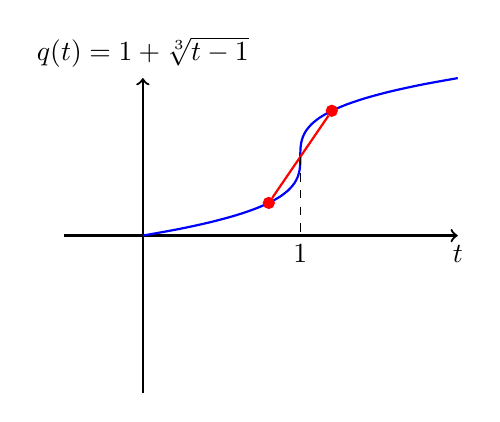
\begin{tikzpicture}
[
	closedpt/.style={circle,draw,fill,inner sep=0pt,minimum size=4pt},
	openpt/.style={circle,draw,inner sep=0pt,minimum size=4pt},
	yscale=1,
	xscale=2
]

	% v0 = 30, g = 10

	% axes
	\draw[->,thick] (\xmin,0) -- (\xmax,0) node[below] {$t$};
	\draw[->,thick] (0,\ymin) -- (0,\ymax) node[above] {$q(t) = 1 + \sqrt[3]{t - 1}$};

	% position
	\draw[blue,thick,domain=-1:1,smooth,rotate=90,xscale=-1,xshift=-1cm,yshift=-1cm] plot (\x,{ \x * \x * \x});

	\node[closedpt,red] at (0.8,0.415) (start) {};
	\node[closedpt,red] at (1.2,1.585) (end) {};
	\draw[thick,red] (start) -- (end);

	% \node[closedpt,green!33!black] at (1.72,13.717) (start) {};
	% \node[closedpt,green!33!black] at (2.22,22.676) (end) {};
	% \draw[thick,green!33!black] (start) -- (end);

	% \node[closedpt,purple] at (1.78,20.661) (start) {};
	% \node[closedpt,purple] at (2.22,20.661) (end) {};
	% \draw[thick,purple] (start) -- (end);

	\draw[dashed, very thin] (1,1) -- (1,0) node[below] {$1$};

\end{tikzpicture}
